\section{Computation skeletons}
%
In this section we define a simple structure which we term a computation
skeleton. The purpose of a computational skeleton is to compactly describe
a feed-forward computation from an input to an output. A single skeleton encompasses a family of neural networks
that share the same skeletal structure. Likewise, it defines a
corresponding kernel space.
%
\begin{definition} A {\em computation skeleton} $\cs$ is a DAG whose
non-input nodes are labeled by activations.
\end{definition}
%
Though the formal definition of neural networks and skeletons appear
identical, we make a conceptual distinction between them as their role in
our analysis is rather different. Accompanied by a set of weights, a neural
network describes a concrete function, whereas the skeleton stands for a
topology common to several networks as well as for a kernel.
To further underscore the differences we note that skeletons are naturally more compact than networks. In particular, all examples of
skeletons in this paper are {\em irreducible}, meaning that for
each two nodes $v,u\in{}V(\cs)$, $\IN(v)\neq\IN(u)$.
We further restrict our attention
to skeletons with a single output node, showing later that single-output
skeletons can capture supervised problems with outputs in $\reals^k$. We
denote by $|\cs|$ the number of non-input nodes of $\cs$.

\begin{figure}[t]
\begin{center}
\begin{tikzpicture}
\foreach \i in {1,...,4}
{
	\draw (\i -7,0) rectangle (\i-7+0.5,0.5);
	\draw [->] (\i-7 +0.25  ,0.5) -- (-4.25 ,1);
}
\draw (-4.5,1) rectangle (-4,1.5);
\draw [->] (-4.25 ,1.5) -- (-4.25 ,2);
\node[text width=3cm] at (-2.85,-0.25) {$\cs_1$};
\foreach \i in {1,...,4}
{
	\draw (\i -1,0) rectangle (\i-1+0.5,0.5);
}
\foreach \i in {1,...,3}
{
	\draw (\i-1 + 0.5 ,1) rectangle (\i-1+1,1.5);
	\draw [->] (\i-1 +0.25  ,0.5) -- (\i-1 + 0.75 ,1);
	\draw [->] (\i-1 +1.25  ,0.5) -- (\i-1 + 0.75 ,1);
	\draw [->] (\i-1 + 0.75 ,1.5) -- (1.75 ,2);
}
\draw (1.5 ,2) rectangle (2,2.5);
\draw [->] (1.75 ,2.5) -- (1.75 ,3);
\node[text width=3cm] at (3.15,-0.25) {$\cs_2$};
\end{tikzpicture}
%
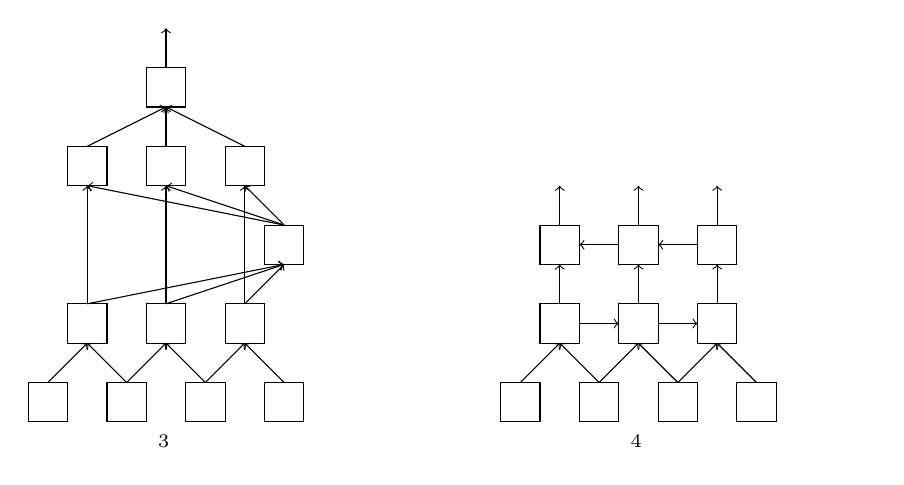
\begin{tikzpicture}
\foreach \i in {1,...,4}
{
	\draw (\i -7,0) rectangle (\i-7+0.5,0.5);
}
\foreach \i in {1,...,3}
{
	\draw (\i-7 + 0.5 ,1) rectangle (\i-7+1,1.5);
	\draw [->] (\i-7 +0.25  ,0.5) -- (\i-7 + 0.75 ,1);
	\draw [->] (\i-7 +1.25  ,0.5) -- (\i-7 + 0.75 ,1);
	\draw [->] (\i-7 + 0.75 ,1.5) -- (-2.75 ,2);
}
\draw (-3 ,2) rectangle (-2.5,2.5);
\foreach \i in {1,...,3}
{
	\draw (\i-7 + 0.5 ,3) rectangle (\i-7+1,3.5);
	\draw [->] (\i-7 +0.75, 1.5) -- (\i-7 +0.75,3);
	\draw [->] (-2.75, 2.5) -- (\i-7 +0.75,3);
	\draw [->] (\i-7 + 0.75 ,3.5) -- (-4.25 ,4);
}
\draw (-4.5 ,4) rectangle (-4,4.5);
\draw [->] (-4.25 ,4.5) -- (-4.25 ,5);
\node[text width=3cm] at (-2.85,-0.25) {$\cs_3$};
\foreach \i in {1,...,4}
{
	\draw (\i -1,0) rectangle (\i-1+0.5,0.5);
}
\foreach \i in {1,...,3}
{
	\draw (\i-1 + 0.5 ,1) rectangle (\i-1+1,1.5);
	\draw [->] (\i-1 +0.25  ,0.5) -- (\i-1 + 0.75 ,1);
	\draw [->] (\i-1 +1.25  ,0.5) -- (\i-1 + 0.75 ,1);
	\draw [->] (\i-1 + 0.75 ,1.5) -- (\i-1 + 0.75 ,2);
}
\draw [->] (1 ,1.25) -- (1.5 ,1.25);
\draw [->] (2 ,1.25) -- (2.5 ,1.25);
\foreach \i in {1,...,3}
{
	\draw (\i-1 + 0.5 ,2) rectangle (\i-1+1,2.5);
	\draw [->] (\i-1 + 0.75 ,2.5) -- (\i-1 + 0.75 ,3);
}
\draw [->] (1.5 ,2.25) -- (1 ,2.25);
\draw [->] (2.5 ,2.25) -- (2 ,2.25);
\node[text width=3cm] at (3.15,-0.25) {$\cs_4$};
\end{tikzpicture}
\caption{Examples of computation skeletons.\label{fig:cs_examples}}
\end{center}
\end{figure}

Figure \ref{fig:cs_examples} shows four example skeletons, omitting
the designation of the activation functions. The skeleton
$\cs_1$ is rather basic as it aggregates all the inputs in a single
step. Such topology can be useful in the absence of any prior
knowledge of how the output label may be computed from an input example, and
it is commonly used in natural language processing where the input is
represented as a bag-of-words~\cite{harris1954distributional}. The only structure in $\cs_1$
is a single {\em fully connected} layer:
\begin{terminology}[Fully connected layer of a skeleton]
%
An induced subgraph of a skeleton with $r+1$ nodes, $u_1,\ldots,u_r,v$, is
called a {\em fully connected layer} if its edges are
$u_1v,\ldots,u_rv$.
%
\end{terminology}
The skeleton $\cs_2$ is slightly more involved: it first processes
consecutive (overlapping) parts of the input, and the next layer
aggregates the partial results. Altogether, it corresponds to networks
with a single one-dimensional convolutional layer, followed by a fully
connected layer. The two-dimensional (and deeper) counterparts of such skeletons
correspond to networks that are common in visual object recognition.
\begin{terminology}[Convolution layer of a skeleton]
%
Let $s,w,q$ be positive integers and denote $n=s(q-1)+w$. A subgraph
of a skeleton is a one dimensional {\em convolution layer} of width $w$ and stride $s$
if it has $n+q$ nodes, $u_1,\ldots,u_{n}, v_1,\ldots,v_q$, and $q w$ edges,
$u_{s(i-1)+j}\,v_{i}$, for $1\le i\le q,1\le j\le w$.
%
\end{terminology}
%% The skeleton $\cs_3$ is a somewhat more sophisticated version of $\cs_2$, in
%% which after the local computations, a global computation is carried out
%% through a single aggregation node. The local computations are then
%% reassessed and finally aggregated again. The last skeleton, $\cs_4$, can be
%% useful for learning sequence-to-sequence mappings and similar skeletons
%% often used in translation, speech recognition, and OCR tasks.
The skeleton $\cs_3$ is a somewhat more sophisticated version of $\cs_2$: the local computations are first aggregated, then reconsidered with the aggregate, and finally aggregated again.
%
The last skeleton, $\cs_4$, corresponds to the networks that arise in
learning sequence-to-sequence mappings as used in translation, speech
recognition, and OCR tasks (see for example~\citet{sutskever2014sequence}).

\subsection{From computation skeletons to neural networks}
%
%% We are now ready to describe how a skeleton when accompanied with a
The following definition shows how a skeleton, accompanied with a
replication parameter $r\ge 1$ and a number of output nodes $k$,
induces a neural network architecture. Recall that inputs are ordered
sets of vectors in $\sphere^{d-1}$.
%% For brevity, we omit $d$ from the
%% notation introduced in the following definition.
%
\begin{definition}[Realization of a skeleton]
%
Let $\cs$ be a computation skeleton and consider input coordinates in
$\sphere^{d-1}$ as in \eqref{eq:coordinates}. For $r, k \ge 1$ we
define the following neural network $\cn=\cn(\cs,r,k)$.
%
For each input node in $\cs$, $\cn$ has $d$ corresponding input
neurons with weight $1/d$. For each internal node $v\in \cs$ labeled by an activation
$\sigma$, $\cn$ has $r$ neurons $v^1,\ldots,v^r$, each with an
activation $\sigma$ and weight $1/r$. In addition, $\cn$ has $k$ output neurons
$o_1,\ldots,o_k$ with the identity activation $\sigma(x)=x$ and weight $1$.
%
There is an edge $v^iu^j\in E(\cn)$ whenever $uv\in
E(\cs)$.  For every output node $v$ in $\cs$, each neuron $v^j$ is
connected to all output neurons $o_1,\ldots,o_k$. We term $\cn$ the
{\em $(r,k)$-fold realization} of $\cs$. We also define the {\em $r$-fold realization} of $\cs$ as\footnote{Note that for every $k$,
$\netrep\left(\cn(\cs,r,1)\right)=\netrep\left(\cn(\cs,r,k)\right)$.} $\cn(\cs,r)= \netrep\left(\cn(\cs,r,1)\right)$.
%
\end{definition}

%
\noindent
Note that the notion of the replication parameter $r$ corresponds, in
the terminology of convolutional networks, to the number of
channels taken in a convolutional layer and to the number of hidden units
taken in a fully-connected layer.
%% We would like to note that the architectures obtained by realizations of
%% skeletons include naturally many of the standard architectures employed in
%% practice such as fully connected layers, in which $r$ corresponds to the
%% number of hidden neurons, and convolutional layers, in which $r$ corresponds
%% to the number of channels.

Figure~\ref{fig:ct_to_nn} illustrates a $(5,4)$- and $5$-realizations
of a skeleton with coordinate dimension $d=2$.  The
$(5,4)$-realization is a network with a single (one dimensional)
convolutional layer having $5$ channels, stride of $2$, and width of
$4$, followed by three fully-connected layers. The global replication
parameter $r$ in a realization is used for brevity; it is
straightforward to extend results when the different nodes in $\cs$
are each replicated to a different extent.

%% We would also like to note that
%% for brevity, we use same replication parameter $r$ for all nodes. It is
%% straightforward to extend the definition and the results presented
%% henceforth to the case when different nodes in $\cs$ are associated with
%% different replication values.

\begin{figure}[t]
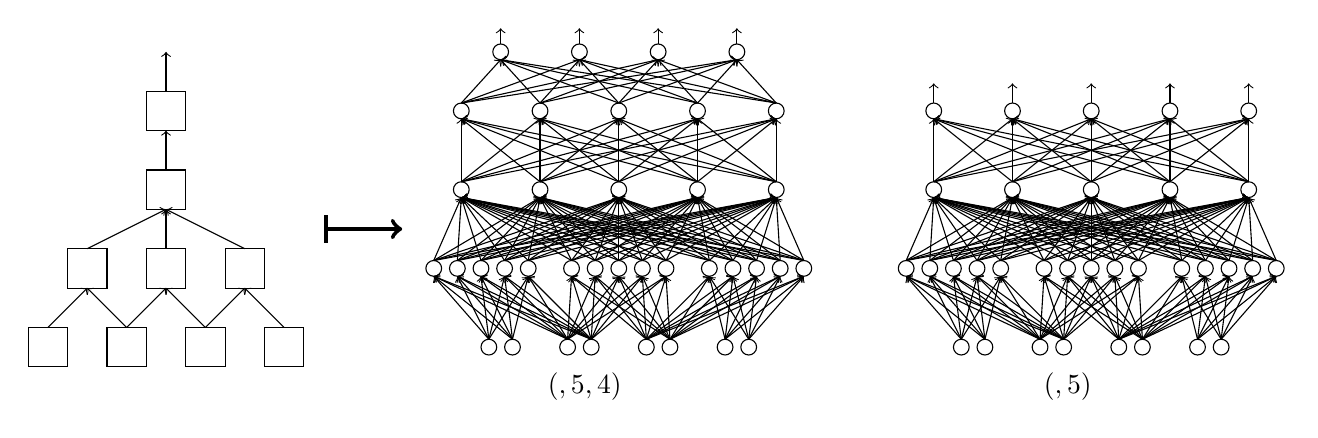
\begin{tikzpicture}
\foreach \i in {1,...,4}
{
	\draw (\i -1,0) rectangle (\i-1+0.5,0.5);
}
\foreach \i in {1,...,3}
{
	\draw (\i-1 + 0.5 ,1) rectangle (\i-1+1,1.5);
	\draw [->] (\i-1 +0.25  ,0.5) -- (\i-1 + 0.75 ,1);
	\draw [->] (\i-1 +1.25  ,0.5) -- (\i-1 + 0.75 ,1);
	\draw [->] (\i-1 + 0.75 ,1.5) -- (1.75 ,2);
}
\draw (1.5 ,2) rectangle (2,2.5);
\draw [->] (1.75 ,2.5) -- (1.75 ,3);
\draw (1.5 ,3) rectangle (2,3.5);
\draw [->] (1.75 ,3.5) -- (1.75 ,4);
\node[text width=3cm] at (3.15,-0.25) {$\cs$};
\draw [ultra thick, |->] (3.75,1.75) -- (4.75,1.75);
\foreach \i in {1,...,4}
{
	\draw (4.85+\i,0.25) circle [radius=0.1];
	\draw (5.15+\i,0.25) circle [radius=0.1];
}
\foreach \i in {-1,...,1}
{
	\foreach \j in {-2,...,2}
	{
		\draw (7.5+1.75*\i + 0.3*\j,1.25) circle [radius=0.1];
		\draw [->] (6.85+\i,0.35) -- (7.5+1.75*\i + 0.3*\j,1.15);
		\draw [->] (7.15+\i,0.35) -- (7.5+1.75*\i + 0.3*\j,1.15);

		\draw [->] (7.85+\i,0.35) -- (7.5+1.75*\i + 0.3*\j,1.15);
		\draw [->] (8.15+\i,0.35) -- (7.5+1.75*\i + 0.3*\j,1.15);
		\foreach \k in {-2,...,2}
		{
			\draw [->] (7.5+1.75*\i + 0.3*\j,1.35) -- (7.5+\k,2.15);
		}
	}
}
\foreach \j in {-2,...,2}
{
	\draw (7.5+\j,2.25) circle [radius=0.1];
	\foreach \k in {-2,...,2}
	{
		\draw[->] (7.5+\j,2.35) -- (7.5+\k,3.15);
	}
}
\foreach \j in {-2,...,2}
{
	\draw (7.5+\j,3.25) circle [radius=0.1];
	\draw[->] (7.5+\j,3.35) -- (6,3.9);
	\draw[->] (7.5+\j,3.35) -- (7,3.9);
	\draw[->] (7.5+\j,3.35) -- (8,3.9);
	\draw[->] (7.5+\j,3.35) -- (9,3.9);
}
\draw (6,4) circle [radius=0.1];
\draw (7,4) circle [radius=0.1];
\draw (8,4) circle [radius=0.1];
\draw (9,4) circle [radius=0.1];
\draw[->] (6,4.1) -- (6,4.3);
\draw[->] (7,4.1) -- (7,4.3);
\draw[->] (8,4.1) -- (8,4.3);
\draw[->] (9,4.1) -- (9,4.3);
\node[text width=3cm] at (8.1,-0.25) {$\cn(\cs,5,4)$};
\foreach \i in {1,...,4}
{
	\draw (10.85+\i,0.25) circle [radius=0.1];
	\draw (11.15+\i,0.25) circle [radius=0.1];
}
\foreach \i in {-1,...,1}
{
	\foreach \j in {-2,...,2}
	{
		\draw (6+7.5+1.75*\i + 0.3*\j,1.25) circle [radius=0.1];
		\draw [->] (6+6.85+\i,0.35) -- (6+7.5+1.75*\i + 0.3*\j,1.15);
		\draw [->] (6+7.15+\i,0.35) -- (6+7.5+1.75*\i + 0.3*\j,1.15);

		\draw [->] (6+7.85+\i,0.35) -- (6+7.5+1.75*\i + 0.3*\j,1.15);
		\draw [->] (6+8.15+\i,0.35) -- (6+7.5+1.75*\i + 0.3*\j,1.15);
		\foreach \k in {-2,...,2}
		{
			\draw [->] (6+7.5+1.75*\i + 0.3*\j,1.35) -- (6+7.5+\k,2.15);
		}
	}
}
\foreach \j in {-2,...,2}
{
	\draw (6+7.5+\j,2.25) circle [radius=0.1];
	\foreach \k in {-2,...,2}
	{
		\draw[->] (6+7.5+\j,2.35) -- (6+7.5+\k,3.15);
	}
}
\foreach \j in {-2,...,2}
{
	\draw (6+7.5+\j,3.25) circle [radius=0.1];
	\draw[->] (6+7.5+\j,3.35) -- (6+7.5+\j,3.6);
}
\node[text width=3cm] at (6+8.4,-0.25) {$\cn(\cs,5)$};
\end{tikzpicture}
\caption{A $(5,4)$-fold and $5$-fold realizations of the computation
skeleton $\cs$ with $d=2$.\label{fig:ct_to_nn}}
\end{figure}

We next define a scheme for random initialization of the weights of a neural
network, that is similar to what is often done in practice. We employ the definition throughout the paper whenever we refer to
random weights.
%
\begin{definition}[Random weights]\label{def:rand_weights}
%
A {\em random initialization} of a neural network $\cn$ is a
multivariate Gaussian $\w=(w_{uv})_{uv\in E(\cn)}$ such that each weight
$w_{uv}$ is sampled independently from a normal distribution with mean $0$
and variance\footnote{For $U\subset V(\cn)$ we denote $\delta(U) = \sum_{u\in U}\delta(u)$.} ${d\delta(u)}/{\delta(\IN(v))}$ if $u$ is an input neuron and ${\delta(u)}/{\left(\|\sigma_{u}\|^2\,\delta(\IN(v))\right)}$ otherwise.
%
\end{definition}
%
%% In practice, weights are often sampled independently from
%% normal distributions with variance proportional to ${1}/{|\IN(v)|}$.
%% We would like to note that in many architectures, such as convolutional nets,
\noindent
Architectures such as convolutional nets have weights that are shared
across different edges.
% (i.e.\ the same weight is associated with different edges)
Again, it is straightforward to extend our results to these cases and for
simplicity we assume no explicit weight sharing.

\subsection{From computation skeletons to reproducing kernels}
%
In addition to networks' architectures, a computation skeleton $\cs$ also
defines a normalized kernel $\kappa_\cs:\cx\times\cx\to[-1,1]$ and a
corresponding norm $\|\cdot \|_{\cs}$ on functions $f:\cx\to\reals$. This
norm has the property that $\|f\|_{\cs}$ is small if and only if $f$ can be
obtained by certain simple compositions of functions according to the
structure of $\cs$. To define the kernel,
we introduce a {\em dual activation} and {\em dual kernel}. For
$\rho\in[-1,1]$, we denote by $\gaussian_\rho$ the multivariate Gaussian
distribution on $\reals^2$ with mean $0$ and covariance matrix
$\left( \begin{smallmatrix} 1 & \rho \\ \rho & 1 \end{smallmatrix} \right)$.
%% whose diagonal elements are $1$ and off-diagonal elements are $\rho$.
%% \iffalse
%% $\begin{pmatrix} 1 & \rho \\ \rho & 1 \end{pmatrix}$.
%% \fi
%

\begin{definition}[Dual activation and kernel]\label{def:dual_act}
%
The {\em dual activation} of an activation $\sigma$ is the function
$\hat{\sigma}:[-1,1]\to\reals$ defined as
$$
\hat\sigma(\rho) =
	\E_{(X,Y) \sim \gaussian_\rho}\sigma(X)\sigma(Y) \,.
$$
The {\em dual kernel} w.r.t.\ to a Hilbert space $\ch$ is the kernel
$\kappa_\sigma:\ch^1\times \ch^1\to\reals$ defined as
$$\kappa_\sigma(\x,\y) = \hat{\sigma}(\inner{\x,\y}_\ch) \,.$$

%
\end{definition}
%
\noindent
Section~\ref{sec:comp_ker} shows that $\kappa_\sigma$ is indeed a kernel for every activation
$\sigma$ that adheres with the square-integrability requirement.
%
In fact,
any continuous $\mu:[-1,1]\to\reals$, such that
$(\x,\y)\mapsto\mu(\inner{\x,\y}_\ch)$ is a kernel for all $\ch$, is
the dual of some activation.
%
Note that $\kappa_\sigma$ is normalized iff $\sigma$ is normalized.
%
We show in Section~\ref{dualact:sec} that dual activations are closely
related to Hermite polynomial expansions, and that these can be used
to calculate the duals of activation functions analytically.
%
Table~\ref{tab:duals} lists a few examples of normalized activations
and their corresponding dual (corresponding derivations are in
Section~\ref{dualact:sec}).
%
{\renewcommand{\arraystretch}{1.3}%
\begin{table}[t]
\begin{center}
  \begin{tabular}{lllll}
    \hline
    Activation &  & Dual Activation & Kernel & Ref \\ \hline
    Identity & $x$ & $\rho$ & linear\\
    2nd Hermite & $\frac{x^2 - 1}{\sqrt{2}}$ & $\rho^2$ & poly &\\
    ReLU & $\sqrt{2}\,[x]_+$ &
		$\frac{1}{\pi}+\frac{\rho}{2} +
		 \frac{\rho^2}{2\pi} +
		 \frac{\rho^4}{24\pi} + \ldots
		 = \frac{\sqrt{1-\rho^2}+(\pi-\cos^{-1}(\rho))\rho}{\pi}$ &
		 $\arccos_1$  & \cite{cho2009kernel}\\
    Step & $\sqrt{2}\,\ind[{x\ge 0}]$ &
			$\frac{1}{2} +
			 \frac{\rho}{\pi} +
			 \frac{\rho^3}{6\pi} +
			 \frac{3\rho^5}{40\pi} + \ldots = \frac{\pi-\cos^{-1}(\rho)}{\pi}$ &
			 $\arccos_0$ & \cite{cho2009kernel}\\
    Exponential & $e^{x-2}$ &
			$\frac{1}{e}+\frac{\rho}{e}+\frac{\rho^2}{2e}+\frac{\rho^3}{6e}+\ldots=
			e^{\rho-1}$ & RBF & \cite{mairal2014convolutional}\\
			& & & & \vspace{-16pt} \\
			\hline
  \end{tabular}
\caption{Activation functions and their duals.\label{tab:duals}}
\end{center}
\end{table}
}
%
The following definition gives the kernel corresponding to a skeleton
having normalized activations.\footnote{For a skeleton $\cs$ with unnormalized
  activations, the corresponding kernel is the kernel of the skeleton
  $\cs'$ obtained by normalizing the activations of $\cs$.}
%
\begin{definition}[Compositional kernels]\label{def:comp_ker}
%
Let $\cs$ be a computation skeleton with normalized activations and
(single) output node $o$.
%
For every node $v$, inductively define a kernel
$\kappa_v:\cx\times\cx\to\reals$ as follows.
%
For an input node $v$ corresponding to the $i$th coordinate,
define $\kappa_{v}(\x,\y)=\inner{\x^i, \y^i}$.
%
For a non-input node $v$, define
$$
\kappa_v(\x,\y) =
	\hat\sigma_v\left(
		\frac{\sum_{u\in \IN(v)}\kappa_{u}(\x,\y)}{|\IN(v)|}\right) \,.
    $$
The final kernel $\kappa_\cs$ is $\kappa_o$, the kernel associated with
the output node $o$. The resulting Hilbert space and norm are
denoted $\ch_\cs$ and $\|\cdot\|_\cs$ respectively, and
$\ch_v$ and $\|\cdot\|_v$ denote the space and norm when formed at node $v$.
\end{definition}
%
\noindent As we show later, $\kappa_\cs$ is indeed a (normalized) kernel for every
skeleton $\cs$. To understand the kernel in the context of learning, we need
to examine which functions can be expressed as moderate
norm functions in $\ch_\cs$. As we show in section \ref{sec:comp_ker},
these are the functions obtained by certain simple compositions according to the
feed-forward structure of $\cs$. For intuition, the following example
contrasts two commonly used skeletons.

\begin{example}[Convolutional vs.\ fully connected skeletons]
\label{exam:diff_struct}
Consider a network whose activations are all ReLU, $\sigma(z)=[z]_+$,
and an input space $\cx_{n,1}=\{\pm 1\}^n$. Say that $\cs_1$ is a
skeleton comprising a single fully connected layer, and that $\cs_2$ is one comprising
a convolutional layer of stride $1$ and width $q=\log^{0.999}(n)$, followed by a single fully-connected layer. (The skeleton $\cs_2$ from
Figure~\ref{fig:cs_examples} is a concrete example of the convolutional
skeleton with $q=2$ and $n=4$.)
%
The kernel $\kappa_{\cs_1}$ takes the form $\kappa_{\cs_1}(\x,\y) =
\hat{\sigma} \left({\inner{\x,\y}}/{n}\right)$. It is a symmetric kernel and
therefore functions with small norm in $\ch_{\cs_1}$ are essentially
low-degree polynomials. For instance, fix a bound $R=n^{1.001}$ on the norm
of the functions.
In this case, the space $\ch^{R}_{\cs_1}$ contains
multiplication of one or two input coordinates. However, multiplication of
$3$ or more coordinates are no-longer in $\ch^{R}_{\cs_1}$. Moreover, this
property holds true regardless of the choice of activation
function. On the other hand, $\ch^{R}_{\cs_2}$ contains functions
whose dependence on adjacent input coordinates is far more complex. It includes,
for instance, any function $f:\cx\to \{\pm 1\}$ that is symmetric
(i.e.\ $f(x)=f(-x)$) and that depends on $q$ adjacent coordinates
$\x_{i},\ldots,\x_{i+q}$. Furthermore, any sum of $n$ such functions is
also in $\ch^{R}_{\cs_2}$.
\end{example}
